\chapter{Introducción}



\section{Problemática y motivación}

La almendra es la fruta seca de mayor producción y consumo en el mundo.~\autocite{iannamico:frutossecos} Se comercializa con diversos grados de industrialización: con cáscara; pelada; blanqueada; en trozos; como harina; como aceite y como pasta, entre otros. El mercado mundial de las almendras está dominado en un \SI{80}{\percent} por dos principales productores: Estados Unidos y España. En \num{2015}, nuestro país tenía más de \num{4000} hectáreas cultivadas (ver tabla \ref{tabla:supcultivada}), siendo Mendoza la provincia de mayor superficie cultivada, seguida por San Juan y La Rioja. En \num{2013} se importaron más de \num{1800} toneladas de almendras para el consumo local —desde Chile y Estados Unidos—, mientras que se exportaron \num{33} toneladas a España, Paraguay y Uruguay.~\autocite{faostat}


\begin{table}[hbt]
\centering
\caption[Cultivos de almendra en Argentina en 2015]{cultivos de almendra en Argentina en 2015.~\autocite{iannamico:cultivo}}
\label{tabla:supcultivada}
\begin{tabular}{@{}lr@{}}
\toprule
Provincia           & Superficie cultivada {[}Ha{]} \\ \cmidrule{1-2} % o \midrule
Mendoza             & 2580                          \\
San Juan            & 572                           \\
La Rioja            & 498                           \\
Salta               & 189                           \\
Río Negro y Neuquén & 170                           \\
Otras               & 200                           \\
Total               & 4209                          \\ \bottomrule
\end{tabular}
\end{table}


El procesamiento mínimo para comercializar las almendras implica el descapotado y el pelado. El descapotado consiste en eliminar la cáscara externa o \enquote{capote} (exocarpio y mesocarpio del fruto); en el pelado se rompe la cáscara interna (endocarpio del fruto) para finalmente extraer la semilla. Este procesamiento es realizado mecánicamente por máquinas especializadas, pero puede provocar ligeros daños en algunos frutos. Posteriormente se realiza un proceso de clasificación o filtrado en el cual se eliminan restos de cáscaras, almendras dañadas y cualquier objeto extraño. Esta clasificación es habitualmente realizada mediante clasificadores ópticos, máquinas de alta tecnología y costo que mediante iluminadores, cámaras y eyectores de aire, separan los productos buenos de los malos y la basura.

En la región, y particularmente en la provincia de San Juan, la producción está centrada en pequeñas y medianas empresas agroindustriales. Hoy en día algunos productores optan por vender las almendras con cáscara; serán otros quienes les den, al pelarlas, mayor valor agregado. Otros productores sí realizan esa etapa de procesado, separando las almendras buenas de forma manual, lo cual requiere mano de obra especializada y muchas horas de trabajo; el promedio por operario es de entre \num{15} y \SI{30}{\kg} por jornada. La escasez de mano de obra especializada (debido a lo rutinario de la tarea) impacta en los costos de producción, pero estos productores no pueden afrontar los costos de adquirir una máquina clasificadora óptica.

El \nombre{Proyecto de Desarrollo Tecnológico y Social} (\nombre{PDTS}) \enquote{Diseño e implementación de una estrategia de clasificación óptica de almendras para pequeños productores} es una iniciativa impulsada por la \nombre{Universidad Nacional de San Juan} (\nombre{UNSJ}) y la \nombre{Secretaría de Ciencia, Tecnología e Innovación} del \nombre{Gobierno de San Juan} (\nombre{SECITI}) que pretende, a largo plazo, desarrollar una clasificadora óptica de almendras destinada al sector \nombre{MiPyME} agroindustrial de la región del Nuevo Cuyo.~\autocite{pdts} Para ello hay que diseñar, construir y probar todas las partes mecánicas, electrónicas y de software de la máquina, como así también los procesos que en ella se realizan y cómo se integran a los procesos existentes. Debe ser de bajo costo y ser al menos tan eficiente como un operario humano que clasifica manualmente.

Este trabajo es un pequeño aporte inicial a ese \nombre{PDTS}, y aborda el diseño e implementación de un sistema de visión artificial para la clasificación de almendras




\section{La almendra}
La almendra es el fruto (tipo drupa) del árbol llamado almendro (\textit{Prunus dulcis [Mill.] D.A.Webb}). Una drupa es un fruto monospermo de mesocarpio carnoso, coriáceo o fibroso, que rodea a un endocarpio leñoso (carozo o hueso) con una sola semilla en su interior. Otras drupas son el durazno, la cereza, la aceituna y el café.

En la almendra el mesocarpio y el exocarpio forman la parte más blanda, correosa, del fruto; se conoce como cáscara o capote (en inglés: \ingles{hull}). El endocarpio (ver figura \ref{fig:partesalmendra}) es la cáscara dura, carozo o hueso (en inglés: \ingles{shell}). En la parte interna del carozo está la semilla (\ingles{kernel}) dicotiledónea, que es lo que vulgarmente se conoce como almendra. Esta se puede dividir longitudinalmente en dos mitades llamadas cotiledones. La semilla tiene una piel marrón que la rodea: el tegumento. Para diferenciar las partes de la semilla, llamaremos \enquote{carne} a la parte blanca que está dentro del tegumento.


\begin{figure}[hbtp]
\centering
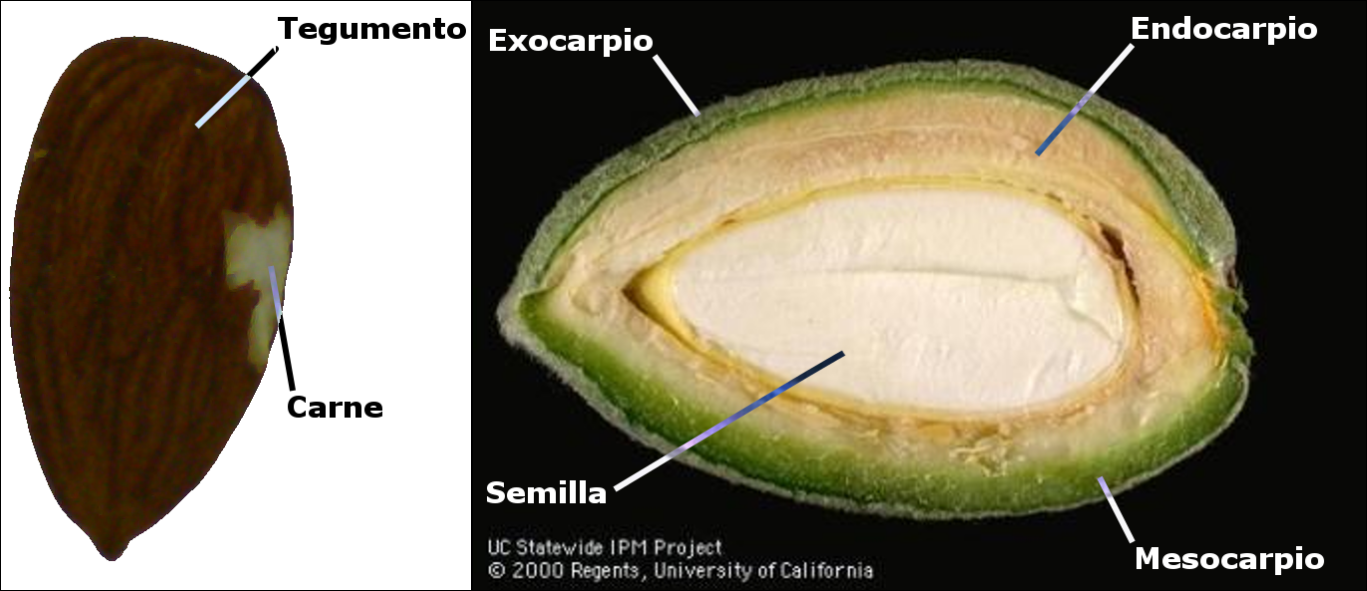
\includegraphics[width=\imagengrande]{almendra_partes_1_2}
\caption[Partes de una almendra]{partes de una almendra. Izquierda: semilla; derecha: corte de un fruto completo.~\autocite[][]{imagenes:interioralmendra}}
\label{fig:partesalmendra}
\end{figure}




\section{Normas}
Existen normas que regulan el comercio de almendras peladas (sin cáscara). Hay tres normas que fueron útiles para definir los defectos a encontrar: 
\begin{enumerate}
\item la Resolución \num{1352/1967} (capítulos XV y XIX) de la antigua \nombre{Secretaría de Agricultura y Ganadería de la República Argentina}, hoy bajo la órbita del \nombre{Servicio Nacional de Sanidad y Calidad Agroalimentaria} (\nombre{SENASA});~\autocite{standards:res1352}

\item el \enquote{Estándar estadounidense para la calidad de almendras peladas}, elaborado por el \nombre{Departamento de Agricultura} de ese país (\nombre{USDA});~\autocite{standards:usda}

\item el \enquote{Estándar DDP-06 acerca de la comercialización y control de calidad comercial de semillas de almendra}, elaborado por la \nombre{Comisión Económica de las Naciones Unidas para Europa} (\nombre{UNECE}).~\autocite{standards:unece}

\end{enumerate}

Los tres documentos definen rasgos generales sobre los bienes a comercializar, y caracterizan defectos a encontrar, como \enquote{almendras partidas}, \enquote{almendras dobles}, \enquote{moho}, \enquote{fragmento} y otros. Por último, establecen clases de calidad, cada una con distinta tolerancia a defectos o variaciones.

Las normas de \nombre{UNECE} y \nombre{USDA} son más explícitas a la hora de definir los defectos que la norma de \nombre{SENASA}. El \nombre{Código Alimentario Argentino} replica en su capítulo XI una versión abreviada de la Resolución \num{1352/1967}.~\autocite{codigoalimentario}



\section{Soluciones existentes}
Existen en el mercado máquinas capaces de resolver el problema con el mismo enfoque; se denominan máquinas de clasificación óptica o seleccionadoras ópticas (en inglés es común denominarlas como  \ingles{optical sorting machines}, y no \ingles{optical classification machines}). Se utilizan, en general, luego de etapas de filtrado mecánico. Estas máquinas pueden usarse para una gran cantidad de frutos; el fabricante ajusta sus parámetros y añade o quita componentes según el fruto a clasificar y el presupuesto del comprador. 

La estructura de la gran mayoría de ellas consiste de:

\begin{enumerate}
\item Una cinta transportadora o plataforma vibradora, que mueve los frutos.
\item Un tobogán o tubo que guía los frutos hacia un espacio de caída libre.
\item Una o más cámaras que capturan imágenes desde uno o ambos lados del objeto.
\item Eyectores que soplan los objetos malos.
\item Salidas de objetos malos y objetos buenos.
\end{enumerate}
A modo de ejemplo, la figura \ref{fig:diagramamaquina} muestra un esquema de funcionamiento de una clasificadora \nombre{Tomra Nimbus}.



\begin{figure}[hbtp]
\centering
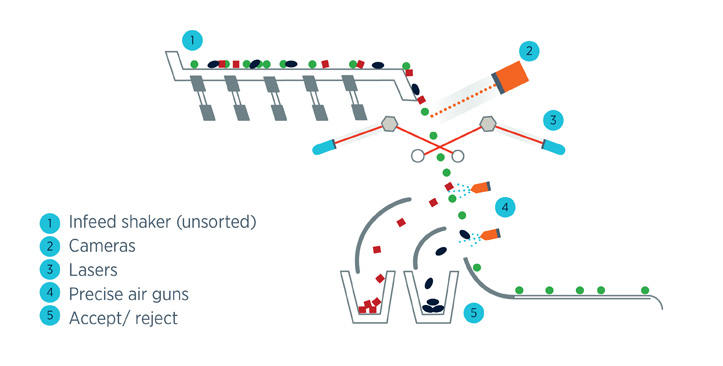
\includegraphics[width=\imagengrande]{tomra_nimbus_diagrama}
\caption[Diagrama de funcionamiento de una máquina comercial]{diagrama de funcionamiento de una máquina \nombre{Tomra Nimbus}.~\autocite{imagenes:nimbusdiagrama}}
\label{fig:diagramamaquina}
\end{figure}
%TODO: Vectorizar.


La figura \ref{fig:salidamaquina} muestra la salida típica de una máquina clasificadora. Los defectos que pueden detectarse están determinados por el software de las máquinas y por el sistema de visión que tienen. Respecto a esto último, pueden tener cámaras e iluminadores en el espectro visible, en ultravioleta y en infrarrojo, que permiten detectar:
\begin{itemize}
\item Problemas de forma;
\item Problemas de color;
\item Hongos y toxinas superficiales;
\item Objetos extraños.
\end{itemize}



\begin{figure}[hbtp]
\centering
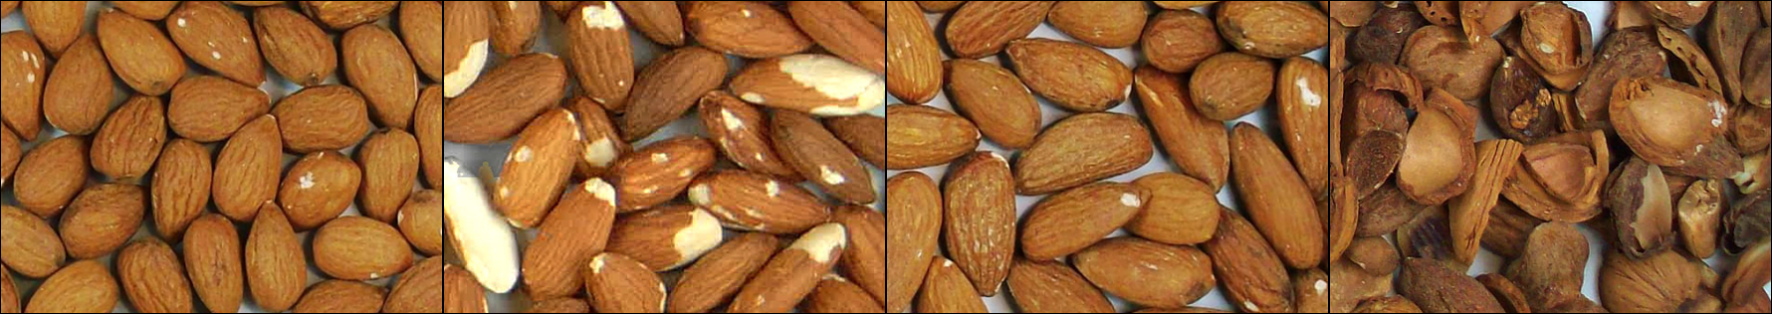
\includegraphics[width=\imagengrande]{almendras_clasificadora_a}
\caption[Salida de una máquina clasificadora comercial]{salida de una máquina clasificadora comercial. De izquierda a derecha: almendras aceptadas; rechazadas por astilladas o raspadas; rechazadas por tamaño; rechazadas por ser cáscaras, almendras manchadas o podridas.~\autocite{imagenes:almendrasclasificadas}}
\label{fig:salidamaquina}
\end{figure}


La mayoría usa sensores CCD e iluminadores led, pero algunas incorporan luz láser y los sensores correspondientes, para analizar ciertos defectos. 

Algunas empresas que fabrican estas máquinas son \nombre{Tomra}, \nombre{Bühler}, \nombre{Cimbria} y \nombre{Key Technology}; algunas de sus máquinas se muestran en la figura \ref{fig:maquinas}. Hay muchas más que fabrican máquinas simples que solo analizan el color. No se encontró información respecto a la precisión de las máquinas. Su capacidad depende del producto a analizar y los defectos a encontrar, pero es mayor a \SI{0,5}{toneladas/hora}, pudiendo alcanzar \SI{15}{toneladas/hora}.

En nuestro país, las máquinas de la familia \nombre{Sortex} de \nombre{Bühler} tienen un costo que oscila entre los \SI{100000}{USD} y los \SI{300000}{USD} ---alrededor de \SI{1780000}{ARS} y \SI{5340000}{ARS} respectivamente, en agosto de 2017---, dependiendo de los defectos a remover y la capacidad de producción (entre \num{2} y \SI{15}{toneladas/hora}). En función de esto varían el tipo y cantidad de cámaras (entre dos y veinte).\footnote{Según comunicación por correo electrónico con \nombre{Walter Tosco} de \nombre{Bühler Sortex Argentina} (\url{http://sortex.com.ar}).}



\begin{figure}[hbtp]
\centering
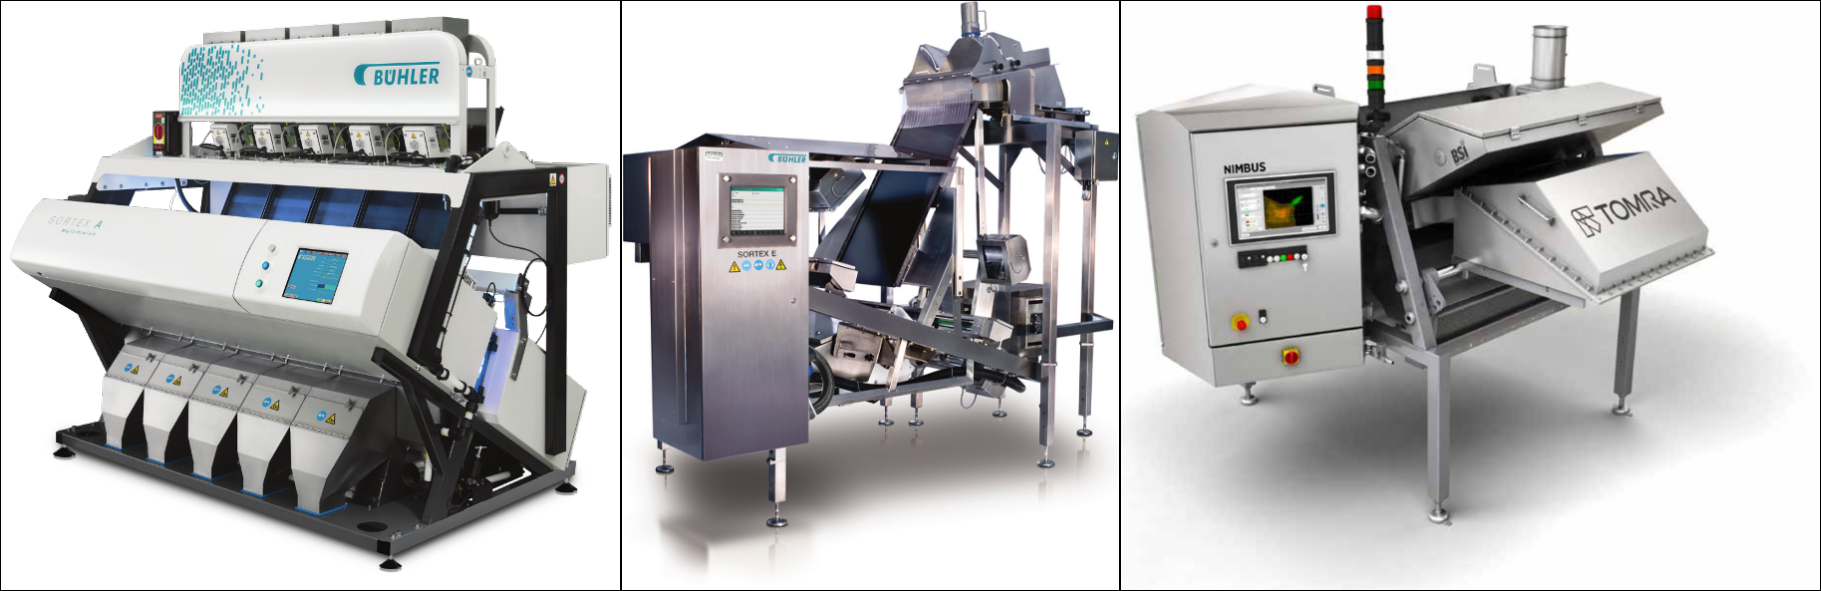
\includegraphics[width=\imagengrande]{maquinas}
\caption[Máquinas clasificadoras]{máquinas clasificadoras ópticas. De izquierda a derecha: \nombre{Bühler Sortex A}, \nombre{Bühler Sortex E}, \nombre{Tomra Nimbus}.~\autocite{imagenes:maquinasbuhler,imagenes:maquinastomra}}
\label{fig:maquinas}
\end{figure}



\section{Propuesta}
En este trabajo se quisieron abordar tres áreas específicas de la máquina: el software de clasificación, el proceso de captura y el sistema de desplazamiento de las almendras. Una vez comenzado el trabajo se hizo evidente que el sistema de visión artificial necesario no es independiente de los mecanismos de traslación y eyección de objetos. Dado que estos últimos no están definidos todavía (y dependen de otras partes del proceso), adoptar un subsistema de visión único, sin considerar posibles limitaciones a las otras partes del sistema clasificador, es una decisión que probablemente implicaría problemas en futuras etapas. Es por esto que se decidió:

\begin{enumerate}
\item Hacer pruebas cortas de posibles sistemas de visión, lo más genéricos posibles.
\item Tomar el que mejor funcione (según algún criterio) y utilizarlo para generar un gran conjunto de imágenes.
\end{enumerate}

Este conjunto de imágenes se usa para evaluar la efectividad que tienen diversos descriptores o predictores para clasificar los objetos que ingresen al sistema. Algunos de los descriptores usados son propuestos en la literatura revisada, mientras que otros surgen de nuestro análisis del problema de clasificación. Análogamente, se prueban diversas formas de identificar de forma unívoca las posiciones y límites de los objetos en las imágenes —tarea conocida como segmentación—.

El conjunto de imágenes fue generado a partir de almendras y otros objetos provistos por un productor local. Se utilizaron (parcialmente) las normas de \nombre{UNECE} como verdad o patrón de referencia, para definir los defectos a buscar en las almendras y para comparar los resultados obtenidos. Algunos valores de referencia, como el color y el tamaño, se determinan a partir de la muestra ya que son características que varían naturalmente entre especies y cosechas.



\section{Herramientas y materiales}\label{intro:herramientasymateriales}
Se resumen a continuación algunas de las herramientas y materiales que se utilizaron en este trabajo. Se extenderá su descripción y forma de uso en secciones posteriores.

\begin{enumerate}
\item Cámara web \nombre{Genius eFace 2050AF}.
\item Muestras  de almendras y otros objetos, provistos por el productor.
\item \nombre{Matlab R2015b}~\autocite{soft:matlab}. Se decidió hacer el desarrollo de los algoritmos en \nombre{Matlab}, ya que es una herramienta versátil; buena para la experimentación y el análisis; y de amplio uso en el \nombre{Instituto de Automática} (\nombre{INAUT}), donde probablemente se continúe el desarrollo del sistema.

Cajas de herramientas usadas:
	\begin{enumerate}
	\item {\nombre{Image Processing Toolbox}}
	\item {\nombre{Computer Vision System Toolbox}}
	\item {\nombre{Image Acquisition Toolbox}}
	\item {\nombre{Statistics and Machine Learning Toolbox}}
	\end{enumerate}
Otros:
	\begin{enumerate}
	\item {\nombre{Matlab Support Package for USB Webcams}}
	\item \nombre{YAMLMatlab}, para trabajar con archivos YAML de configuración de parámetros~\autocite{soft:yamlmatlab}
	\item \nombre{MBeautifier}, para uniformar el formato del código~\autocite{soft:mbeautifier}
	\item \nombre{multic} ({\nombre{Confusion Matrix and its Derivations}})~\autocite{soft:multic}
	\item {\nombre{Balu Toolbox for Matlab}}~\autocite{soft:balu}
	\end{enumerate}
\item \nombre{GIMP 2.8.18}:  Programa de edición de imágenes utilizado como complemento a \nombre{Matlab} para el diseño de algoritmos y análisis de las imágenes disponibles. Se usó también el complemento \nombre{G’MIC 1.79} para el procesamiento.~\autocite{soft:gimp,soft:gmic}
\item \nombre{KNIME 3.3.2}: Programa de minería de datos usado para comparar resultados.~\autocite{soft:knime}
\item Perfiles metálicos y accesorios; poliestireno de alto impacto; madera MDF; vidrios y espejos, para la construcción de un prototipo de estructura.
\item Tiras de leds, una fuente conmutada y materiales eléctricos, para la construcción de luminarias.
\end{enumerate}
